% Content for DWT Methods subsection
% This file is included in the main conference paper via % Content for DWT Methods subsection
% This file is included in the main conference paper via % Content for DWT Methods subsection
% This file is included in the main conference paper via % Content for DWT Methods subsection
% This file is included in the main conference paper via \input{DWTMethods}

The Discrete Wavelet Transform (DWT) is a powerful transform coding technique that decomposes signals into a hierarchy of resolution levels, making it particularly well-suited for image compression. In this work we focus on the Haar wavelet, which is the simplest in the family of wavelets used for this transform. For now on we consider an image as a 1D signal, we later discuss how to convert it to 2D.

\subsubsection{One Dimensional Haar Wavelet Transform in Practice}

Consider a 1D signal with $2^k$ values: $$ \{x_1, x_2, \dots, x_{2^k}\}$$ A naive approach to compression might be to store only the average of adjacent values, resulting in the compressed signal $$A_{k-1} = \{(x_1 + x_2) / 2, (x_3 + x_4) / 2, \dots, (x_{2^k-1} + x_{2^k})/2\}$$ Note that this approach clearly loses information. To enable perfect reconstruction of the original signal, we must also preserve the difference between adjacent values: $$D_{k-1} = \{x_1 - (x_1 + x_2) / 2, x_3 - (x_3 + x_4) / 2, \dots\}$$
Note that the difference of $x_i$ the the mean is completely symmetric to the difference of $x_{i+1}$ to the mean, so we only need to store one detail coefficient. This simple idea is the core of the Haar wavelet transform.

We can apply this operation once and we get a set of $2^k/2$ average coefficients and $2^k/2$ detail coefficients. We can keep applying the operation recursively to the average coefficients until we reach only one pixel of average coefficient. Table~\ref{tab:haar_decomposition} illustrates this process for an 8-pixel signal.

Figure~\ref{fig:haar_decomposition} visualizes this decomposition process, showing the signal (blue) and wavelets (red) at each resolution level. The blue curves represent the averaged signals at decreasing resolutions, while the red curves capture the detail coefficients (differences) that must be preserved for perfect reconstruction.

\begin{table}[h]
  \centering
  \caption{Haar decomposition example for an 8-pixel signal}
  \label{tab:haar_decomposition}
  \begin{tabular}{c c c}
    \toprule
    \textbf{Resolution} & \textbf{Averages} & \textbf{Details} \\
    \midrule
    8 & $[5, \; 8, \; 9, \; 7, \; 4, \; 2, \; 1, \; 3]$ & --- \\
    4 & $[6.5, \; 8, \; 3, \; 2]$ & $[-1.5, \; 1, \; 1, \; -1]$ \\
    2 & $[7.25, \; 2.5]$ & $[-0.75, \; 0.5]$ \\
    1 & $[4.875]$ & $[2.375]$ \\
    \bottomrule
  \end{tabular}
\end{table}

\begin{figure}[ht]
  \centering
  \input{methods/DWTdiagrams/haar_decomposition}
  \caption{Haar wavelet decomposition showing signal (blue) and wavelets (red) at each resolution level.}
  \label{fig:haar_decomposition}
\end{figure}

Note that for a given level we can perfectly reconstruct the previous level's average coefficients from the combination of the average coefficient and detail coefficients, so all we need to store in a compression is the set of all detail coefficients and the very last average.

\subsubsection{Theoretical Foundation for Haar Wavelet Transform}

The Haar wavelet transform is founded on a set of nested vector spaces $V^j$ representing piecewise-constant functions at different resolutions, where $V^0 \subset V^1 \subset V^2 \subset \dots$. This nested structure enables a change of basis from the natural basis of scaling functions in $V^{j+1}$ to a basis consisting of the scaling functions from the lower-resolution space $V^j$ together with the wavelet basis functions from the orthogonal complement space $W^j$. The scaling functions provide the coarse approximation, while the wavelets capture the detail information needed for perfect reconstruction. Figure~\ref{fig:basis_functions} visualizes the scaling functions and Haar wavelets for different resolution levels.

\begin{figure*}[hbt]
  \centering
  \begin{minipage}{\textwidth}
    \centering
    \input{methods/DWTdiagrams/scaling_functions}
    \subcaption{Scaling functions (basis) for $V^3$: eight piecewise constant functions.}
    \label{fig:scaling_functions}
  \end{minipage}
  \vspace{0.5cm}
  \begin{minipage}{\textwidth}
    \centering
    \input{methods/DWTdiagrams/wavelet_basis}
    \subcaption{Basis for $V^2$ (blue) and Haar wavelets basis for $W^2$ (red).}
    \label{fig:wavelet_basis}
  \end{minipage}
  \caption{Haar basis: scaling functions for $V^3$ and scaling functions and wavelets for $V^2$ and $W^2$.}
  \label{fig:basis_functions}
\end{figure*}

A detailed mathematical exposition of the vector space structure, scaling functions, inner products, orthogonality, and the Haar wavelet basis functions is provided in Appendix \ref{apx:haartheory}.




\subsubsection{Two-Dimensional Haar Wavelet Transform}

The 2D Haar wavelet transform generalizes the 1D "averaging and differencing" filter bank to 2D by alternating between operations on rows and columns at each level of the hierarchy.

\paragraph{The Decomposition Algorithm}

The algorithm proceeds recursively as follows:

\begin{enumerate}
\item \textbf{Row Step:} First, perform one step of horizontal pairwise averaging and differencing on the pixel values in each row of the image. This splits the image horizontally into averages (left) and details (right).

\item \textbf{Column Step:} Next, apply vertical pairwise averaging and differencing to each column of the result from the Row Step.
\begin{itemize}
\item This creates four distinct quadrants of coefficients:
\begin{itemize}
\item \textbf{Top-Left:} Averages of averages (coarse approximation).
\item \textbf{Top-Right:} Averages of horizontal details.
\item \textbf{Bottom-Left:} Vertical details of horizontal averages.
\item \textbf{Bottom-Right:} Vertical details of horizontal details (diagonal details).
\end{itemize}
\end{itemize}

\item \textbf{Recursion:} To complete the transformation, repeat this process recursively \textit{only} on the quadrant containing the averages in both directions (the top-left quadrant).
\end{enumerate}

Figure~\ref{fig:encoded_visualization} visualizes this 2D Haar transform decomposition process, showing how an image is decomposed into four quadrants at each level.

\begin{figure}[ht]
  \centering
  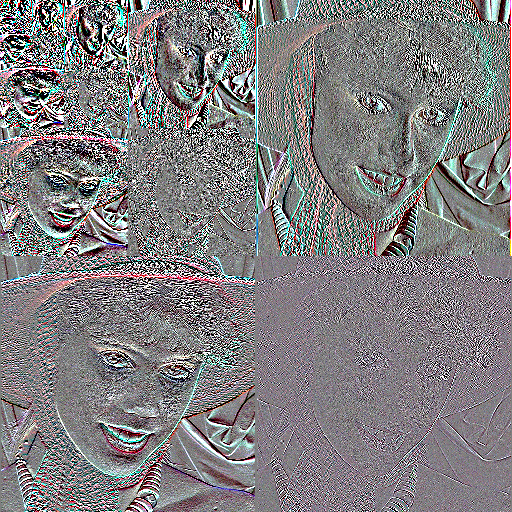
\includegraphics[width=0.3\textwidth]{methods/DWTdiagrams/encodedVisualization.png}
  \caption{Visualization of a 2D Haar transform showing the decomposition of an image}
  \label{fig:encoded_visualization}
\end{figure}




\subsubsection{Compression Properties}

The Haar wavelet transform is particularly effective for image compression because it naturally concentrates energy in the low-resolution approximation coefficients. The detail coefficients (wavelets) typically have smaller magnitudes and can be more aggressively quantized or discarded in lossy compression scenarios. This energy compaction property, combined with the transform's computational efficiency makes the Haar wavelet an attractive choice for practical image compression systems.



The Discrete Wavelet Transform (DWT) is a powerful transform coding technique that decomposes signals into a hierarchy of resolution levels, making it particularly well-suited for image compression. In this work we focus on the Haar wavelet, which is the simplest in the family of wavelets used for this transform. For now on we consider an image as a 1D signal, we later discuss how to convert it to 2D.

\subsubsection{One Dimensional Haar Wavelet Transform in Practice}

Consider a 1D signal with $2^k$ values: $$ \{x_1, x_2, \dots, x_{2^k}\}$$ A naive approach to compression might be to store only the average of adjacent values, resulting in the compressed signal $$A_{k-1} = \{(x_1 + x_2) / 2, (x_3 + x_4) / 2, \dots, (x_{2^k-1} + x_{2^k})/2\}$$ Note that this approach clearly loses information. To enable perfect reconstruction of the original signal, we must also preserve the difference between adjacent values: $$D_{k-1} = \{x_1 - (x_1 + x_2) / 2, x_3 - (x_3 + x_4) / 2, \dots\}$$
Note that the difference of $x_i$ the the mean is completely symmetric to the difference of $x_{i+1}$ to the mean, so we only need to store one detail coefficient. This simple idea is the core of the Haar wavelet transform.

We can apply this operation once and we get a set of $2^k/2$ average coefficients and $2^k/2$ detail coefficients. We can keep applying the operation recursively to the average coefficients until we reach only one pixel of average coefficient. Table~\ref{tab:haar_decomposition} illustrates this process for an 8-pixel signal.

Figure~\ref{fig:haar_decomposition} visualizes this decomposition process, showing the signal (blue) and wavelets (red) at each resolution level. The blue curves represent the averaged signals at decreasing resolutions, while the red curves capture the detail coefficients (differences) that must be preserved for perfect reconstruction.

\begin{table}[h]
  \centering
  \caption{Haar decomposition example for an 8-pixel signal}
  \label{tab:haar_decomposition}
  \begin{tabular}{c c c}
    \toprule
    \textbf{Resolution} & \textbf{Averages} & \textbf{Details} \\
    \midrule
    8 & $[5, \; 8, \; 9, \; 7, \; 4, \; 2, \; 1, \; 3]$ & --- \\
    4 & $[6.5, \; 8, \; 3, \; 2]$ & $[-1.5, \; 1, \; 1, \; -1]$ \\
    2 & $[7.25, \; 2.5]$ & $[-0.75, \; 0.5]$ \\
    1 & $[4.875]$ & $[2.375]$ \\
    \bottomrule
  \end{tabular}
\end{table}

\begin{figure}[ht]
  \centering
  % Haar wavelet decomposition diagram showing signal and wavelets at each resolution level
% Arranged in a 2x2 grid to fit in a single column
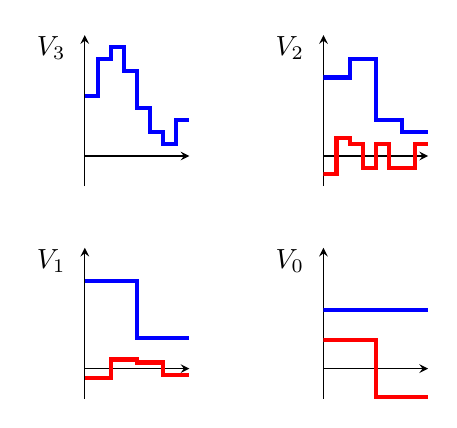
\begin{tikzpicture}
  % Top row: Resolution 8 (V_3) - top left
  \begin{axis}[
    at={(0.13\textwidth,4.5cm)},
    width=0.24\textwidth,
    height=3.5cm,
    xmin=0, xmax=1,
    ymin=-2.5, ymax=10,
    ytick=\empty,
    xtick=\empty,
    axis x line=middle,
    axis y line=center,
  ]
    \addplot[const plot, line width=1.5pt, color=blue] coordinates {
      (0,5) (0.125,5) (0.125,8) (0.25,8) (0.25,9) (0.375,9) (0.375,7) (0.5,7) (0.5,4) (0.625,4) (0.625,2) (0.75,2) (0.75,1) (0.875,1) (0.875,3) (1,3)
    };
  \end{axis}
  \node[anchor=east] at (0.12\textwidth, 6.25cm) {$V_3$};
  
  % Top row: Resolution 4 (V_2) - top right
  \begin{axis}[
    at={(0.38\textwidth,4.5cm)},
    width=0.24\textwidth,
    height=3.5cm,
    xmin=0, xmax=1,
    ymin=-2.5, ymax=10,
    ytick=\empty,
    xtick=\empty,
    axis x line=middle,
    axis y line=center,
  ]
    \addplot[const plot, line width=1.5pt, color=blue] coordinates {
      (0,6.5) (0.25,6.5) (0.25,8) (0.5,8) (0.5,3) (0.75,3) (0.75,2) (1,2)
    };
    \addplot[const plot, line width=1.5pt, color=red] coordinates {
      (0,-1.5) (0.125,-1.5) (0.125,1.5) (0.25,1.5) (0.25,1) (0.375,1) (0.375,-1) (0.5,-1) (0.5,1) (0.625,1) (0.625,-1) (0.75,-1) (0.75,-1) (0.875,-1) (0.875,1) (1,1)
    };
  \end{axis}
  \node[anchor=east] at (0.37\textwidth, 6.25cm) {$V_2$};

  % Bottom row: Resolution 2 (V_1) - bottom left
  \begin{axis}[
    at={(0.13\textwidth,1.8cm)},
    width=0.24\textwidth,
    height=3.5cm,
    xmin=0, xmax=1,
    ymin=-2.5, ymax=10,
    ytick=\empty,
    xtick=\empty,
    axis x line=middle,
    axis y line=center,
  ]
    \addplot[const plot, line width=1.5pt, color=blue] coordinates {
      (0,7.25) (0.5,7.25) (0.5,2.5) (1,2.5)
    };
    \addplot[const plot, line width=1.5pt, color=red] coordinates {
      (0,-0.75) (0.25,-0.75) (0.25,0.75) (0.5,0.75) (0.5,0.5) (0.75,0.5) (0.75,-0.5) (1,-0.5)
    };
  \end{axis}
  \node[anchor=east] at (0.12\textwidth, 3.55cm) {$V_1$};
  
  % Bottom row: Resolution 1 (V_0) - bottom right
  \begin{axis}[
    at={(0.38\textwidth,1.8cm)},
    width=0.24\textwidth,
    height=3.5cm,
    xmin=0, xmax=1,
    ymin=-2.5, ymax=10,
    ytick=\empty,
    xtick=\empty,
    axis x line=middle,
    axis y line=center,
  ]
    \addplot[const plot, line width=1.5pt, color=blue] coordinates {
      (0,4.875) (1,4.875)
    };
    \addplot[const plot, line width=1.5pt, color=red] coordinates {
      (0,2.375) (0.5,2.375) (0.5,-2.375) (1,-2.375)
    };
  \end{axis}
  \node[anchor=east] at (0.37\textwidth, 3.55cm) {$V_0$};

\end{tikzpicture}


  \caption{Haar wavelet decomposition showing signal (blue) and wavelets (red) at each resolution level.}
  \label{fig:haar_decomposition}
\end{figure}

Note that for a given level we can perfectly reconstruct the previous level's average coefficients from the combination of the average coefficient and detail coefficients, so all we need to store in a compression is the set of all detail coefficients and the very last average.

\subsubsection{Theoretical Foundation for Haar Wavelet Transform}

The Haar wavelet transform is founded on a set of nested vector spaces $V^j$ representing piecewise-constant functions at different resolutions, where $V^0 \subset V^1 \subset V^2 \subset \dots$. This nested structure enables a change of basis from the natural basis of scaling functions in $V^{j+1}$ to a basis consisting of the scaling functions from the lower-resolution space $V^j$ together with the wavelet basis functions from the orthogonal complement space $W^j$. The scaling functions provide the coarse approximation, while the wavelets capture the detail information needed for perfect reconstruction. Figure~\ref{fig:basis_functions} visualizes the scaling functions and Haar wavelets for different resolution levels.

\begin{figure*}[hbt]
  \centering
  \begin{minipage}{\textwidth}
    \centering
    % Scaling functions (basis) for V_3: eight piecewise constant functions
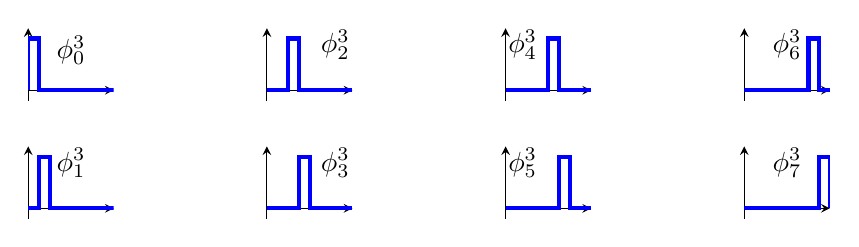
\begin{tikzpicture}
  % Column 1: Scaling functions 1 and 2
  % Scaling function 1: [0, 1/8)
  \begin{axis}[
    at={(0,0)},
    width=0.22\textwidth,
    height=2.5cm,
    xmin=0, xmax=1,
    ymin=-0.2, ymax=1.2,
    ytick=\empty,
    xtick=\empty,
    axis x line=middle,
    axis y line=center,
  ]
    \addplot[const plot, line width=1.5pt, color=blue] coordinates {
      (0,0) (0,1) (0.125,1) (0.125,0) (1,0)
    };
    \node[above] at (0.5, 0.3) {$\phi_0^3$};
  \end{axis}
  % Scaling function 2: [1/8, 1/4)
  \begin{axis}[
    at={(0,-1.5cm)},
    width=0.22\textwidth,
    height=2.5cm,
    xmin=0, xmax=1,
    ymin=-0.2, ymax=1.2,
    ytick=\empty,
    xtick=\empty,
    axis x line=middle,
    axis y line=center,
  ]
    \addplot[const plot, line width=1.5pt, color=blue] coordinates {
      (0,0) (0.125,0) (0.125,1) (0.25,1) (0.25,0) (1,0)
    };
    \node[above] at (0.5, 0.4) {$\phi_1^3$};
  \end{axis}
  
  % Column 2: Scaling functions 3 and 4
  % Scaling function 3: [1/4, 3/8)
  \begin{axis}[
    at={(0.25\textwidth,0)},
    width=0.22\textwidth,
    height=2.5cm,
    xmin=0, xmax=1,
    ymin=-0.2, ymax=1.2,
    ytick=\empty,
    xtick=\empty,
    axis x line=middle,
    axis y line=center,
  ]
    \addplot[const plot, line width=1.5pt, color=blue] coordinates {
      (0,0) (0.25,0) (0.25,1) (0.375,1) (0.375,0) (1,0)
    };
    \node[above] at (0.8, 0.4) {$\phi_2^3$};
  \end{axis}
  % Scaling function 4: [3/8, 1/2)
  \begin{axis}[
    at={(0.25\textwidth,-1.5cm)},
    width=0.22\textwidth,
    height=2.5cm,
    xmin=0, xmax=1,
    ymin=-0.2, ymax=1.2,
    ytick=\empty,
    xtick=\empty,
    axis x line=middle,
    axis y line=center,
  ]
    \addplot[const plot, line width=1.5pt, color=blue] coordinates {
      (0,0) (0.375,0) (0.375,1) (0.5,1) (0.5,0) (1,0)
    };
    \node[above] at (0.8, 0.4) {$\phi_3^3$};
  \end{axis}
  
  % Column 3: Scaling functions 5 and 6
  % Scaling function 5: [1/2, 5/8)
  \begin{axis}[
    at={(0.5\textwidth,0)},
    width=0.22\textwidth,
    height=2.5cm,
    xmin=0, xmax=1,
    ymin=-0.2, ymax=1.2,
    ytick=\empty,
    xtick=\empty,
    axis x line=middle,
    axis y line=center,
  ]
    \addplot[const plot, line width=1.5pt, color=blue] coordinates {
      (0,0) (0.5,0) (0.5,1) (0.625,1) (0.625,0) (1,0)
    };
    \node[above] at (0.2, 0.4) {$\phi_4^3$};
  \end{axis}
  % Scaling function 6: [5/8, 3/4)
  \begin{axis}[
    at={(0.5\textwidth,-1.5cm)},
    width=0.22\textwidth,
    height=2.5cm,
    xmin=0, xmax=1,
    ymin=-0.2, ymax=1.2,
    ytick=\empty,
    xtick=\empty,
    axis x line=middle,
    axis y line=center,
  ]
    \addplot[const plot, line width=1.5pt, color=blue] coordinates {
      (0,0) (0.625,0) (0.625,1) (0.75,1) (0.75,0) (1,0)
    };
    \node[above] at (0.2, 0.4) {$\phi_5^3$};
  \end{axis}
  
  % Column 4: Scaling functions 7 and 8
  % Scaling function 7: [3/4, 7/8)
  \begin{axis}[
    at={(0.75\textwidth,0)},
    width=0.22\textwidth,
    height=2.5cm,
    xmin=0, xmax=1,
    ymin=-0.2, ymax=1.2,
    ytick=\empty,
    xtick=\empty,
    axis x line=middle,
    axis y line=center,
  ]
    \addplot[const plot, line width=1.5pt, color=blue] coordinates {
      (0,0) (0.75,0) (0.75,1) (0.875,1) (0.875,0) (1,0)
    };
    \node[above] at (0.5, 0.4) {$\phi_6^3$};
  \end{axis}
  % Scaling function 8: [7/8, 1)
  \begin{axis}[
    at={(0.75\textwidth,-1.5cm)},
    width=0.22\textwidth,
    height=2.5cm,
    xmin=0, xmax=1,
    ymin=-0.2, ymax=1.2,
    ytick=\empty,
    xtick=\empty,
    axis x line=middle,
    axis y line=center,
  ]
    \addplot[const plot, line width=1.5pt, color=blue] coordinates {
      (0,0) (0.875,0) (0.875,1) (1,1) (1,0)
    };
    \node[above] at (0.5, 0.4) {$\phi_7^3$};
  \end{axis}
\end{tikzpicture}


    \subcaption{Scaling functions (basis) for $V^3$: eight piecewise constant functions.}
    \label{fig:scaling_functions}
  \end{minipage}
  \vspace{0.5cm}
  \begin{minipage}{\textwidth}
    \centering
    % Basis for V_2 (blue) and Haar wavelets basis for W_2 (red)
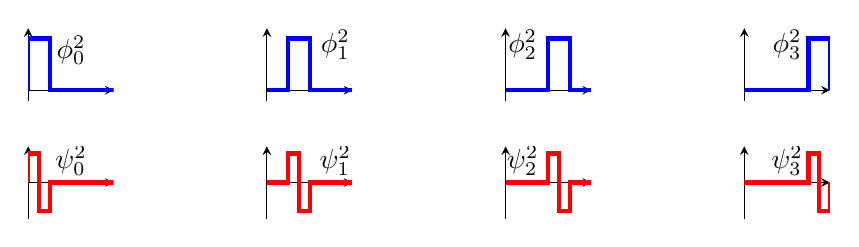
\begin{tikzpicture}
  % V_2 Scaling functions (row above)
  % Scaling function 1: [0, 1/4)
  \begin{axis}[
    at={(0,1.5cm)},
    width=0.22\textwidth,
    height=2.5cm,
    xmin=0, xmax=1,
    ymin=-0.2, ymax=1.2,
    ytick=\empty,
    xtick=\empty,
    axis x line=middle,
    axis y line=center,
  ]
    \addplot[const plot, line width=1.5pt, color=blue] coordinates {
      (0,0) (0,1) (0.25,1) (0.25,0) (1,0)
    };
    \node[above] at (0.5, 0.3) {$\phi_0^2$};
  \end{axis}
  % Scaling function 2: [1/4, 1/2)
  \begin{axis}[
    at={(0.25\textwidth,1.5cm)},
    width=0.22\textwidth,
    height=2.5cm,
    xmin=0, xmax=1,
    ymin=-0.2, ymax=1.2,
    ytick=\empty,
    xtick=\empty,
    axis x line=middle,
    axis y line=center,
  ]
    \addplot[const plot, line width=1.5pt, color=blue] coordinates {
      (0,0) (0.25,0) (0.25,1) (0.5,1) (0.5,0) (1,0)
    };
    \node[above] at (0.8, 0.4) {$\phi_1^2$};
  \end{axis}
  % Scaling function 3: [1/2, 3/4)
  \begin{axis}[
    at={(0.5\textwidth,1.5cm)},
    width=0.22\textwidth,
    height=2.5cm,
    xmin=0, xmax=1,
    ymin=-0.2, ymax=1.2,
    ytick=\empty,
    xtick=\empty,
    axis x line=middle,
    axis y line=center,
  ]
    \addplot[const plot, line width=1.5pt, color=blue] coordinates {
      (0,0) (0.5,0) (0.5,1) (0.75,1) (0.75,0) (1,0)
    };
    \node[above] at (0.2, 0.4) {$\phi_2^2$};
  \end{axis}
  % Scaling function 4: [3/4, 1)
  \begin{axis}[
    at={(0.75\textwidth,1.5cm)},
    width=0.22\textwidth,
    height=2.5cm,
    xmin=0, xmax=1,
    ymin=-0.2, ymax=1.2,
    ytick=\empty,
    xtick=\empty,
    axis x line=middle,
    axis y line=center,
  ]
    \addplot[const plot, line width=1.5pt, color=blue] coordinates {
      (0,0) (0.75,0) (0.75,1) (1,1) (1,0)
    };
    \node[above] at (0.5, 0.4) {$\phi_3^2$};
  \end{axis}
  
  % Wavelet level 2, first: [0, 1/8) vs [1/8, 1/4)
  \begin{axis}[
    at={(0,0)},
    width=0.22\textwidth,
    height=2.5cm,
    xmin=0, xmax=1,
    ymin=-2.5, ymax=2.5,
    ytick=\empty,
    xtick=\empty,
    axis x line=middle,
    axis y line=center,
  ]
    \addplot[const plot, line width=1.5pt, color=red] coordinates {
      (0,0) (0,2) (0.125,2) (0.125,-2) (0.25,-2) (0.25,0) (1,0)
    };
    \node[above] at (0.5, -0.2) {$\psi_0^2$};
  \end{axis}
  % Wavelet level 2, second: [1/4, 3/8) vs [3/8, 1/2)
  \begin{axis}[
    at={(0.25\textwidth,0)},
    width=0.22\textwidth,
    height=2.5cm,
    xmin=0, xmax=1,
    ymin=-2.5, ymax=2.5,
    ytick=\empty,
    xtick=\empty,
    axis x line=middle,
    axis y line=center,
  ]
    \addplot[const plot, line width=1.5pt, color=red] coordinates {
      (0,0) (0.25,0) (0.25,2) (0.375,2) (0.375,-2) (0.5,-2) (0.5,0) (1,0)
    };
    \node[above] at (0.8, -0.2) {$\psi_1^2$};
  \end{axis}
  % Wavelet level 2, third: [1/2, 5/8) vs [5/8, 3/4)
  \begin{axis}[
    at={(0.5\textwidth,0)},
    width=0.22\textwidth,
    height=2.5cm,
    xmin=0, xmax=1,
    ymin=-2.5, ymax=2.5,
    ytick=\empty,
    xtick=\empty,
    axis x line=middle,
    axis y line=center,
  ]
    \addplot[const plot, line width=1.5pt, color=red] coordinates {
      (0,0) (0.5,0) (0.5,2) (0.625,2) (0.625,-2) (0.75,-2) (0.75,0) (1,0)
    };
    \node[above] at (0.2, -0.2) {$\psi_2^2$};
  \end{axis}
  % Wavelet level 2, fourth: [3/4, 7/8) vs [7/8, 1)
  \begin{axis}[
    at={(0.75\textwidth,0)},
    width=0.22\textwidth,
    height=2.5cm,
    xmin=0, xmax=1,
    ymin=-2.5, ymax=2.5,
    ytick=\empty,
    xtick=\empty,
    axis x line=middle,
    axis y line=center,
  ]
    \addplot[const plot, line width=1.5pt, color=red] coordinates {
      (0,0) (0.75,0) (0.75,2) (0.875,2) (0.875,-2) (1,-2) (1,0)
    };
    \node[above] at (0.5, -0.2) {$\psi_3^2$};
  \end{axis}
\end{tikzpicture}


    \subcaption{Basis for $V^2$ (blue) and Haar wavelets basis for $W^2$ (red).}
    \label{fig:wavelet_basis}
  \end{minipage}
  \caption{Haar basis: scaling functions for $V^3$ and scaling functions and wavelets for $V^2$ and $W^2$.}
  \label{fig:basis_functions}
\end{figure*}

A detailed mathematical exposition of the vector space structure, scaling functions, inner products, orthogonality, and the Haar wavelet basis functions is provided in Appendix \ref{apx:haartheory}.




\subsubsection{Two-Dimensional Haar Wavelet Transform}

The 2D Haar wavelet transform generalizes the 1D "averaging and differencing" filter bank to 2D by alternating between operations on rows and columns at each level of the hierarchy.

\paragraph{The Decomposition Algorithm}

The algorithm proceeds recursively as follows:

\begin{enumerate}
\item \textbf{Row Step:} First, perform one step of horizontal pairwise averaging and differencing on the pixel values in each row of the image. This splits the image horizontally into averages (left) and details (right).

\item \textbf{Column Step:} Next, apply vertical pairwise averaging and differencing to each column of the result from the Row Step.
\begin{itemize}
\item This creates four distinct quadrants of coefficients:
\begin{itemize}
\item \textbf{Top-Left:} Averages of averages (coarse approximation).
\item \textbf{Top-Right:} Averages of horizontal details.
\item \textbf{Bottom-Left:} Vertical details of horizontal averages.
\item \textbf{Bottom-Right:} Vertical details of horizontal details (diagonal details).
\end{itemize}
\end{itemize}

\item \textbf{Recursion:} To complete the transformation, repeat this process recursively \textit{only} on the quadrant containing the averages in both directions (the top-left quadrant).
\end{enumerate}

Figure~\ref{fig:encoded_visualization} visualizes this 2D Haar transform decomposition process, showing how an image is decomposed into four quadrants at each level.

\begin{figure}[ht]
  \centering
  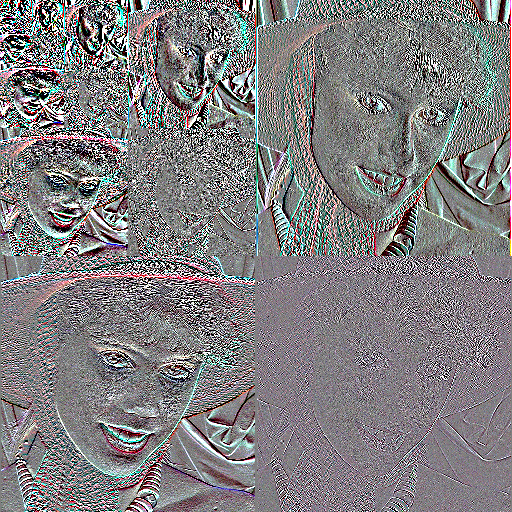
\includegraphics[width=0.3\textwidth]{methods/DWTdiagrams/encodedVisualization.png}
  \caption{Visualization of a 2D Haar transform showing the decomposition of an image}
  \label{fig:encoded_visualization}
\end{figure}




\subsubsection{Compression Properties}

The Haar wavelet transform is particularly effective for image compression because it naturally concentrates energy in the low-resolution approximation coefficients. The detail coefficients (wavelets) typically have smaller magnitudes and can be more aggressively quantized or discarded in lossy compression scenarios. This energy compaction property, combined with the transform's computational efficiency makes the Haar wavelet an attractive choice for practical image compression systems.



The Discrete Wavelet Transform (DWT) is a powerful transform coding technique that decomposes signals into a hierarchy of resolution levels, making it particularly well-suited for image compression. In this work we focus on the Haar wavelet, which is the simplest in the family of wavelets used for this transform. For now on we consider an image as a 1D signal, we later discuss how to convert it to 2D.

\subsubsection{One Dimensional Haar Wavelet Transform in Practice}

Consider a 1D signal with $2^k$ values: $$ \{x_1, x_2, \dots, x_{2^k}\}$$ A naive approach to compression might be to store only the average of adjacent values, resulting in the compressed signal $$A_{k-1} = \{(x_1 + x_2) / 2, (x_3 + x_4) / 2, \dots, (x_{2^k-1} + x_{2^k})/2\}$$ Note that this approach clearly loses information. To enable perfect reconstruction of the original signal, we must also preserve the difference between adjacent values: $$D_{k-1} = \{x_1 - (x_1 + x_2) / 2, x_3 - (x_3 + x_4) / 2, \dots\}$$
Note that the difference of $x_i$ the the mean is completely symmetric to the difference of $x_{i+1}$ to the mean, so we only need to store one detail coefficient. This simple idea is the core of the Haar wavelet transform.

We can apply this operation once and we get a set of $2^k/2$ average coefficients and $2^k/2$ detail coefficients. We can keep applying the operation recursively to the average coefficients until we reach only one pixel of average coefficient. Table~\ref{tab:haar_decomposition} illustrates this process for an 8-pixel signal.

Figure~\ref{fig:haar_decomposition} visualizes this decomposition process, showing the signal (blue) and wavelets (red) at each resolution level. The blue curves represent the averaged signals at decreasing resolutions, while the red curves capture the detail coefficients (differences) that must be preserved for perfect reconstruction.

\begin{table}[h]
  \centering
  \caption{Haar decomposition example for an 8-pixel signal}
  \label{tab:haar_decomposition}
  \begin{tabular}{c c c}
    \toprule
    \textbf{Resolution} & \textbf{Averages} & \textbf{Details} \\
    \midrule
    8 & $[5, \; 8, \; 9, \; 7, \; 4, \; 2, \; 1, \; 3]$ & --- \\
    4 & $[6.5, \; 8, \; 3, \; 2]$ & $[-1.5, \; 1, \; 1, \; -1]$ \\
    2 & $[7.25, \; 2.5]$ & $[-0.75, \; 0.5]$ \\
    1 & $[4.875]$ & $[2.375]$ \\
    \bottomrule
  \end{tabular}
\end{table}

\begin{figure}[ht]
  \centering
  % Haar wavelet decomposition diagram showing signal and wavelets at each resolution level
% Arranged in a 2x2 grid to fit in a single column
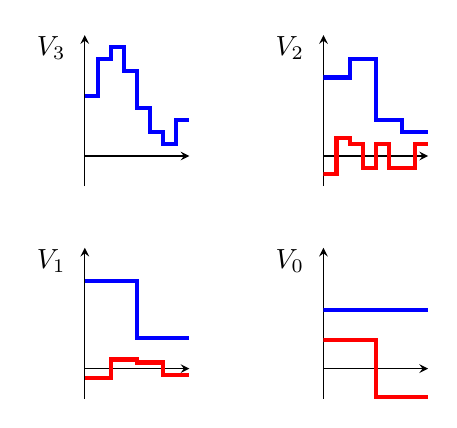
\begin{tikzpicture}
  % Top row: Resolution 8 (V_3) - top left
  \begin{axis}[
    at={(0.13\textwidth,4.5cm)},
    width=0.24\textwidth,
    height=3.5cm,
    xmin=0, xmax=1,
    ymin=-2.5, ymax=10,
    ytick=\empty,
    xtick=\empty,
    axis x line=middle,
    axis y line=center,
  ]
    \addplot[const plot, line width=1.5pt, color=blue] coordinates {
      (0,5) (0.125,5) (0.125,8) (0.25,8) (0.25,9) (0.375,9) (0.375,7) (0.5,7) (0.5,4) (0.625,4) (0.625,2) (0.75,2) (0.75,1) (0.875,1) (0.875,3) (1,3)
    };
  \end{axis}
  \node[anchor=east] at (0.12\textwidth, 6.25cm) {$V_3$};
  
  % Top row: Resolution 4 (V_2) - top right
  \begin{axis}[
    at={(0.38\textwidth,4.5cm)},
    width=0.24\textwidth,
    height=3.5cm,
    xmin=0, xmax=1,
    ymin=-2.5, ymax=10,
    ytick=\empty,
    xtick=\empty,
    axis x line=middle,
    axis y line=center,
  ]
    \addplot[const plot, line width=1.5pt, color=blue] coordinates {
      (0,6.5) (0.25,6.5) (0.25,8) (0.5,8) (0.5,3) (0.75,3) (0.75,2) (1,2)
    };
    \addplot[const plot, line width=1.5pt, color=red] coordinates {
      (0,-1.5) (0.125,-1.5) (0.125,1.5) (0.25,1.5) (0.25,1) (0.375,1) (0.375,-1) (0.5,-1) (0.5,1) (0.625,1) (0.625,-1) (0.75,-1) (0.75,-1) (0.875,-1) (0.875,1) (1,1)
    };
  \end{axis}
  \node[anchor=east] at (0.37\textwidth, 6.25cm) {$V_2$};

  % Bottom row: Resolution 2 (V_1) - bottom left
  \begin{axis}[
    at={(0.13\textwidth,1.8cm)},
    width=0.24\textwidth,
    height=3.5cm,
    xmin=0, xmax=1,
    ymin=-2.5, ymax=10,
    ytick=\empty,
    xtick=\empty,
    axis x line=middle,
    axis y line=center,
  ]
    \addplot[const plot, line width=1.5pt, color=blue] coordinates {
      (0,7.25) (0.5,7.25) (0.5,2.5) (1,2.5)
    };
    \addplot[const plot, line width=1.5pt, color=red] coordinates {
      (0,-0.75) (0.25,-0.75) (0.25,0.75) (0.5,0.75) (0.5,0.5) (0.75,0.5) (0.75,-0.5) (1,-0.5)
    };
  \end{axis}
  \node[anchor=east] at (0.12\textwidth, 3.55cm) {$V_1$};
  
  % Bottom row: Resolution 1 (V_0) - bottom right
  \begin{axis}[
    at={(0.38\textwidth,1.8cm)},
    width=0.24\textwidth,
    height=3.5cm,
    xmin=0, xmax=1,
    ymin=-2.5, ymax=10,
    ytick=\empty,
    xtick=\empty,
    axis x line=middle,
    axis y line=center,
  ]
    \addplot[const plot, line width=1.5pt, color=blue] coordinates {
      (0,4.875) (1,4.875)
    };
    \addplot[const plot, line width=1.5pt, color=red] coordinates {
      (0,2.375) (0.5,2.375) (0.5,-2.375) (1,-2.375)
    };
  \end{axis}
  \node[anchor=east] at (0.37\textwidth, 3.55cm) {$V_0$};

\end{tikzpicture}


  \caption{Haar wavelet decomposition showing signal (blue) and wavelets (red) at each resolution level.}
  \label{fig:haar_decomposition}
\end{figure}

Note that for a given level we can perfectly reconstruct the previous level's average coefficients from the combination of the average coefficient and detail coefficients, so all we need to store in a compression is the set of all detail coefficients and the very last average.

\subsubsection{Theoretical Foundation for Haar Wavelet Transform}

The Haar wavelet transform is founded on a set of nested vector spaces $V^j$ representing piecewise-constant functions at different resolutions, where $V^0 \subset V^1 \subset V^2 \subset \dots$. This nested structure enables a change of basis from the natural basis of scaling functions in $V^{j+1}$ to a basis consisting of the scaling functions from the lower-resolution space $V^j$ together with the wavelet basis functions from the orthogonal complement space $W^j$. The scaling functions provide the coarse approximation, while the wavelets capture the detail information needed for perfect reconstruction. Figure~\ref{fig:basis_functions} visualizes the scaling functions and Haar wavelets for different resolution levels.

\begin{figure*}[hbt]
  \centering
  \begin{minipage}{\textwidth}
    \centering
    % Scaling functions (basis) for V_3: eight piecewise constant functions
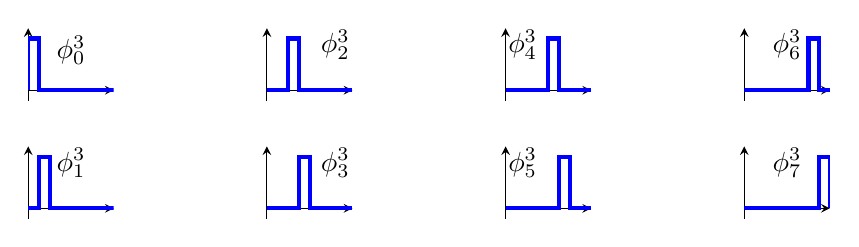
\begin{tikzpicture}
  % Column 1: Scaling functions 1 and 2
  % Scaling function 1: [0, 1/8)
  \begin{axis}[
    at={(0,0)},
    width=0.22\textwidth,
    height=2.5cm,
    xmin=0, xmax=1,
    ymin=-0.2, ymax=1.2,
    ytick=\empty,
    xtick=\empty,
    axis x line=middle,
    axis y line=center,
  ]
    \addplot[const plot, line width=1.5pt, color=blue] coordinates {
      (0,0) (0,1) (0.125,1) (0.125,0) (1,0)
    };
    \node[above] at (0.5, 0.3) {$\phi_0^3$};
  \end{axis}
  % Scaling function 2: [1/8, 1/4)
  \begin{axis}[
    at={(0,-1.5cm)},
    width=0.22\textwidth,
    height=2.5cm,
    xmin=0, xmax=1,
    ymin=-0.2, ymax=1.2,
    ytick=\empty,
    xtick=\empty,
    axis x line=middle,
    axis y line=center,
  ]
    \addplot[const plot, line width=1.5pt, color=blue] coordinates {
      (0,0) (0.125,0) (0.125,1) (0.25,1) (0.25,0) (1,0)
    };
    \node[above] at (0.5, 0.4) {$\phi_1^3$};
  \end{axis}
  
  % Column 2: Scaling functions 3 and 4
  % Scaling function 3: [1/4, 3/8)
  \begin{axis}[
    at={(0.25\textwidth,0)},
    width=0.22\textwidth,
    height=2.5cm,
    xmin=0, xmax=1,
    ymin=-0.2, ymax=1.2,
    ytick=\empty,
    xtick=\empty,
    axis x line=middle,
    axis y line=center,
  ]
    \addplot[const plot, line width=1.5pt, color=blue] coordinates {
      (0,0) (0.25,0) (0.25,1) (0.375,1) (0.375,0) (1,0)
    };
    \node[above] at (0.8, 0.4) {$\phi_2^3$};
  \end{axis}
  % Scaling function 4: [3/8, 1/2)
  \begin{axis}[
    at={(0.25\textwidth,-1.5cm)},
    width=0.22\textwidth,
    height=2.5cm,
    xmin=0, xmax=1,
    ymin=-0.2, ymax=1.2,
    ytick=\empty,
    xtick=\empty,
    axis x line=middle,
    axis y line=center,
  ]
    \addplot[const plot, line width=1.5pt, color=blue] coordinates {
      (0,0) (0.375,0) (0.375,1) (0.5,1) (0.5,0) (1,0)
    };
    \node[above] at (0.8, 0.4) {$\phi_3^3$};
  \end{axis}
  
  % Column 3: Scaling functions 5 and 6
  % Scaling function 5: [1/2, 5/8)
  \begin{axis}[
    at={(0.5\textwidth,0)},
    width=0.22\textwidth,
    height=2.5cm,
    xmin=0, xmax=1,
    ymin=-0.2, ymax=1.2,
    ytick=\empty,
    xtick=\empty,
    axis x line=middle,
    axis y line=center,
  ]
    \addplot[const plot, line width=1.5pt, color=blue] coordinates {
      (0,0) (0.5,0) (0.5,1) (0.625,1) (0.625,0) (1,0)
    };
    \node[above] at (0.2, 0.4) {$\phi_4^3$};
  \end{axis}
  % Scaling function 6: [5/8, 3/4)
  \begin{axis}[
    at={(0.5\textwidth,-1.5cm)},
    width=0.22\textwidth,
    height=2.5cm,
    xmin=0, xmax=1,
    ymin=-0.2, ymax=1.2,
    ytick=\empty,
    xtick=\empty,
    axis x line=middle,
    axis y line=center,
  ]
    \addplot[const plot, line width=1.5pt, color=blue] coordinates {
      (0,0) (0.625,0) (0.625,1) (0.75,1) (0.75,0) (1,0)
    };
    \node[above] at (0.2, 0.4) {$\phi_5^3$};
  \end{axis}
  
  % Column 4: Scaling functions 7 and 8
  % Scaling function 7: [3/4, 7/8)
  \begin{axis}[
    at={(0.75\textwidth,0)},
    width=0.22\textwidth,
    height=2.5cm,
    xmin=0, xmax=1,
    ymin=-0.2, ymax=1.2,
    ytick=\empty,
    xtick=\empty,
    axis x line=middle,
    axis y line=center,
  ]
    \addplot[const plot, line width=1.5pt, color=blue] coordinates {
      (0,0) (0.75,0) (0.75,1) (0.875,1) (0.875,0) (1,0)
    };
    \node[above] at (0.5, 0.4) {$\phi_6^3$};
  \end{axis}
  % Scaling function 8: [7/8, 1)
  \begin{axis}[
    at={(0.75\textwidth,-1.5cm)},
    width=0.22\textwidth,
    height=2.5cm,
    xmin=0, xmax=1,
    ymin=-0.2, ymax=1.2,
    ytick=\empty,
    xtick=\empty,
    axis x line=middle,
    axis y line=center,
  ]
    \addplot[const plot, line width=1.5pt, color=blue] coordinates {
      (0,0) (0.875,0) (0.875,1) (1,1) (1,0)
    };
    \node[above] at (0.5, 0.4) {$\phi_7^3$};
  \end{axis}
\end{tikzpicture}


    \subcaption{Scaling functions (basis) for $V^3$: eight piecewise constant functions.}
    \label{fig:scaling_functions}
  \end{minipage}
  \vspace{0.5cm}
  \begin{minipage}{\textwidth}
    \centering
    % Basis for V_2 (blue) and Haar wavelets basis for W_2 (red)
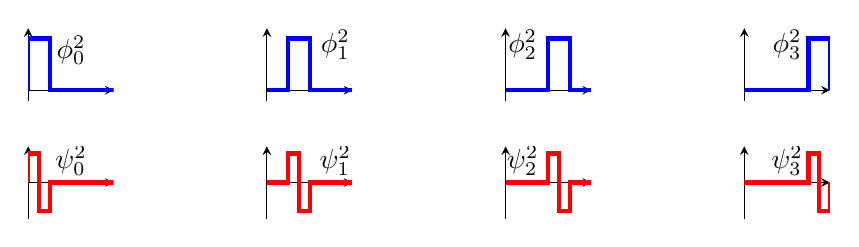
\begin{tikzpicture}
  % V_2 Scaling functions (row above)
  % Scaling function 1: [0, 1/4)
  \begin{axis}[
    at={(0,1.5cm)},
    width=0.22\textwidth,
    height=2.5cm,
    xmin=0, xmax=1,
    ymin=-0.2, ymax=1.2,
    ytick=\empty,
    xtick=\empty,
    axis x line=middle,
    axis y line=center,
  ]
    \addplot[const plot, line width=1.5pt, color=blue] coordinates {
      (0,0) (0,1) (0.25,1) (0.25,0) (1,0)
    };
    \node[above] at (0.5, 0.3) {$\phi_0^2$};
  \end{axis}
  % Scaling function 2: [1/4, 1/2)
  \begin{axis}[
    at={(0.25\textwidth,1.5cm)},
    width=0.22\textwidth,
    height=2.5cm,
    xmin=0, xmax=1,
    ymin=-0.2, ymax=1.2,
    ytick=\empty,
    xtick=\empty,
    axis x line=middle,
    axis y line=center,
  ]
    \addplot[const plot, line width=1.5pt, color=blue] coordinates {
      (0,0) (0.25,0) (0.25,1) (0.5,1) (0.5,0) (1,0)
    };
    \node[above] at (0.8, 0.4) {$\phi_1^2$};
  \end{axis}
  % Scaling function 3: [1/2, 3/4)
  \begin{axis}[
    at={(0.5\textwidth,1.5cm)},
    width=0.22\textwidth,
    height=2.5cm,
    xmin=0, xmax=1,
    ymin=-0.2, ymax=1.2,
    ytick=\empty,
    xtick=\empty,
    axis x line=middle,
    axis y line=center,
  ]
    \addplot[const plot, line width=1.5pt, color=blue] coordinates {
      (0,0) (0.5,0) (0.5,1) (0.75,1) (0.75,0) (1,0)
    };
    \node[above] at (0.2, 0.4) {$\phi_2^2$};
  \end{axis}
  % Scaling function 4: [3/4, 1)
  \begin{axis}[
    at={(0.75\textwidth,1.5cm)},
    width=0.22\textwidth,
    height=2.5cm,
    xmin=0, xmax=1,
    ymin=-0.2, ymax=1.2,
    ytick=\empty,
    xtick=\empty,
    axis x line=middle,
    axis y line=center,
  ]
    \addplot[const plot, line width=1.5pt, color=blue] coordinates {
      (0,0) (0.75,0) (0.75,1) (1,1) (1,0)
    };
    \node[above] at (0.5, 0.4) {$\phi_3^2$};
  \end{axis}
  
  % Wavelet level 2, first: [0, 1/8) vs [1/8, 1/4)
  \begin{axis}[
    at={(0,0)},
    width=0.22\textwidth,
    height=2.5cm,
    xmin=0, xmax=1,
    ymin=-2.5, ymax=2.5,
    ytick=\empty,
    xtick=\empty,
    axis x line=middle,
    axis y line=center,
  ]
    \addplot[const plot, line width=1.5pt, color=red] coordinates {
      (0,0) (0,2) (0.125,2) (0.125,-2) (0.25,-2) (0.25,0) (1,0)
    };
    \node[above] at (0.5, -0.2) {$\psi_0^2$};
  \end{axis}
  % Wavelet level 2, second: [1/4, 3/8) vs [3/8, 1/2)
  \begin{axis}[
    at={(0.25\textwidth,0)},
    width=0.22\textwidth,
    height=2.5cm,
    xmin=0, xmax=1,
    ymin=-2.5, ymax=2.5,
    ytick=\empty,
    xtick=\empty,
    axis x line=middle,
    axis y line=center,
  ]
    \addplot[const plot, line width=1.5pt, color=red] coordinates {
      (0,0) (0.25,0) (0.25,2) (0.375,2) (0.375,-2) (0.5,-2) (0.5,0) (1,0)
    };
    \node[above] at (0.8, -0.2) {$\psi_1^2$};
  \end{axis}
  % Wavelet level 2, third: [1/2, 5/8) vs [5/8, 3/4)
  \begin{axis}[
    at={(0.5\textwidth,0)},
    width=0.22\textwidth,
    height=2.5cm,
    xmin=0, xmax=1,
    ymin=-2.5, ymax=2.5,
    ytick=\empty,
    xtick=\empty,
    axis x line=middle,
    axis y line=center,
  ]
    \addplot[const plot, line width=1.5pt, color=red] coordinates {
      (0,0) (0.5,0) (0.5,2) (0.625,2) (0.625,-2) (0.75,-2) (0.75,0) (1,0)
    };
    \node[above] at (0.2, -0.2) {$\psi_2^2$};
  \end{axis}
  % Wavelet level 2, fourth: [3/4, 7/8) vs [7/8, 1)
  \begin{axis}[
    at={(0.75\textwidth,0)},
    width=0.22\textwidth,
    height=2.5cm,
    xmin=0, xmax=1,
    ymin=-2.5, ymax=2.5,
    ytick=\empty,
    xtick=\empty,
    axis x line=middle,
    axis y line=center,
  ]
    \addplot[const plot, line width=1.5pt, color=red] coordinates {
      (0,0) (0.75,0) (0.75,2) (0.875,2) (0.875,-2) (1,-2) (1,0)
    };
    \node[above] at (0.5, -0.2) {$\psi_3^2$};
  \end{axis}
\end{tikzpicture}


    \subcaption{Basis for $V^2$ (blue) and Haar wavelets basis for $W^2$ (red).}
    \label{fig:wavelet_basis}
  \end{minipage}
  \caption{Haar basis: scaling functions for $V^3$ and scaling functions and wavelets for $V^2$ and $W^2$.}
  \label{fig:basis_functions}
\end{figure*}

A detailed mathematical exposition of the vector space structure, scaling functions, inner products, orthogonality, and the Haar wavelet basis functions is provided in Appendix \ref{apx:haartheory}.




\subsubsection{Two-Dimensional Haar Wavelet Transform}

The 2D Haar wavelet transform generalizes the 1D "averaging and differencing" filter bank to 2D by alternating between operations on rows and columns at each level of the hierarchy.

\paragraph{The Decomposition Algorithm}

The algorithm proceeds recursively as follows:

\begin{enumerate}
\item \textbf{Row Step:} First, perform one step of horizontal pairwise averaging and differencing on the pixel values in each row of the image. This splits the image horizontally into averages (left) and details (right).

\item \textbf{Column Step:} Next, apply vertical pairwise averaging and differencing to each column of the result from the Row Step.
\begin{itemize}
\item This creates four distinct quadrants of coefficients:
\begin{itemize}
\item \textbf{Top-Left:} Averages of averages (coarse approximation).
\item \textbf{Top-Right:} Averages of horizontal details.
\item \textbf{Bottom-Left:} Vertical details of horizontal averages.
\item \textbf{Bottom-Right:} Vertical details of horizontal details (diagonal details).
\end{itemize}
\end{itemize}

\item \textbf{Recursion:} To complete the transformation, repeat this process recursively \textit{only} on the quadrant containing the averages in both directions (the top-left quadrant).
\end{enumerate}

Figure~\ref{fig:encoded_visualization} visualizes this 2D Haar transform decomposition process, showing how an image is decomposed into four quadrants at each level.

\begin{figure}[ht]
  \centering
  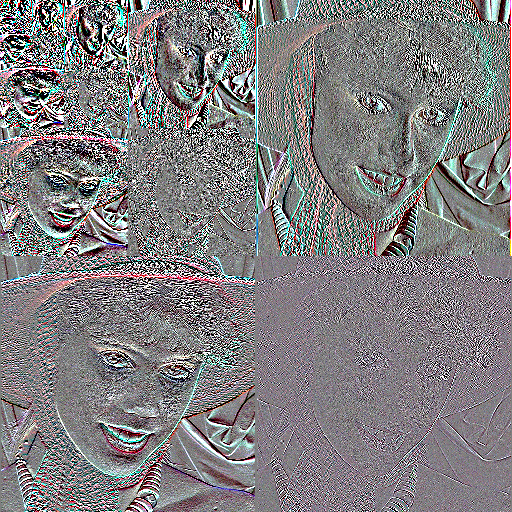
\includegraphics[width=0.3\textwidth]{methods/DWTdiagrams/encodedVisualization.png}
  \caption{Visualization of a 2D Haar transform showing the decomposition of an image}
  \label{fig:encoded_visualization}
\end{figure}




\subsubsection{Compression Properties}

The Haar wavelet transform is particularly effective for image compression because it naturally concentrates energy in the low-resolution approximation coefficients. The detail coefficients (wavelets) typically have smaller magnitudes and can be more aggressively quantized or discarded in lossy compression scenarios. This energy compaction property, combined with the transform's computational efficiency makes the Haar wavelet an attractive choice for practical image compression systems.



The Discrete Wavelet Transform (DWT) is a powerful transform coding technique that decomposes signals into a hierarchy of resolution levels, making it particularly well-suited for image compression. In this work we focus on the Haar wavelet, which is the simplest in the family of wavelets used for this transform. For now on we consider an image as a 1D signal, we later discuss how to convert it to 2D.

\subsubsection{One Dimensional Haar Wavelet Transform in Practice}

Consider a 1D signal with $2^k$ values: $$ \{x_1, x_2, \dots, x_{2^k}\}$$ A naive approach to compression might be to store only the average of adjacent values, resulting in the compressed signal $$A_{k-1} = \{(x_1 + x_2) / 2, (x_3 + x_4) / 2, \dots, (x_{2^k-1} + x_{2^k})/2\}$$ Note that this approach clearly loses information. To enable perfect reconstruction of the original signal, we must also preserve the difference between adjacent values: $$D_{k-1} = \{x_1 - (x_1 + x_2) / 2, x_3 - (x_3 + x_4) / 2, \dots\}$$
Note that the difference of $x_i$ the the mean is completely symmetric to the difference of $x_{i+1}$ to the mean, so we only need to store one detail coefficient. This simple idea is the core of the Haar wavelet transform.

We can apply this operation once and we get a set of $2^k/2$ average coefficients and $2^k/2$ detail coefficients. We can keep applying the operation recursively to the average coefficients until we reach only one pixel of average coefficient. Table~\ref{tab:haar_decomposition} illustrates this process for an 8-pixel signal.

Figure~\ref{fig:haar_decomposition} visualizes this decomposition process, showing the signal (blue) and wavelets (red) at each resolution level. The blue curves represent the averaged signals at decreasing resolutions, while the red curves capture the detail coefficients (differences) that must be preserved for perfect reconstruction.

\begin{table}[h]
  \centering
  \caption{Haar decomposition example for an 8-pixel signal}
  \label{tab:haar_decomposition}
  \begin{tabular}{c c c}
    \toprule
    \textbf{Resolution} & \textbf{Averages} & \textbf{Details} \\
    \midrule
    8 & $[5, \; 8, \; 9, \; 7, \; 4, \; 2, \; 1, \; 3]$ & --- \\
    4 & $[6.5, \; 8, \; 3, \; 2]$ & $[-1.5, \; 1, \; 1, \; -1]$ \\
    2 & $[7.25, \; 2.5]$ & $[-0.75, \; 0.5]$ \\
    1 & $[4.875]$ & $[2.375]$ \\
    \bottomrule
  \end{tabular}
\end{table}

\begin{figure}[ht]
  \centering
  % Haar wavelet decomposition diagram showing signal and wavelets at each resolution level
% Arranged in a 2x2 grid to fit in a single column
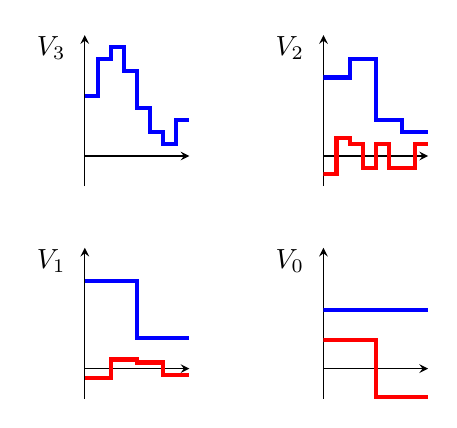
\begin{tikzpicture}
  % Top row: Resolution 8 (V_3) - top left
  \begin{axis}[
    at={(0.13\textwidth,4.5cm)},
    width=0.24\textwidth,
    height=3.5cm,
    xmin=0, xmax=1,
    ymin=-2.5, ymax=10,
    ytick=\empty,
    xtick=\empty,
    axis x line=middle,
    axis y line=center,
  ]
    \addplot[const plot, line width=1.5pt, color=blue] coordinates {
      (0,5) (0.125,5) (0.125,8) (0.25,8) (0.25,9) (0.375,9) (0.375,7) (0.5,7) (0.5,4) (0.625,4) (0.625,2) (0.75,2) (0.75,1) (0.875,1) (0.875,3) (1,3)
    };
  \end{axis}
  \node[anchor=east] at (0.12\textwidth, 6.25cm) {$V_3$};
  
  % Top row: Resolution 4 (V_2) - top right
  \begin{axis}[
    at={(0.38\textwidth,4.5cm)},
    width=0.24\textwidth,
    height=3.5cm,
    xmin=0, xmax=1,
    ymin=-2.5, ymax=10,
    ytick=\empty,
    xtick=\empty,
    axis x line=middle,
    axis y line=center,
  ]
    \addplot[const plot, line width=1.5pt, color=blue] coordinates {
      (0,6.5) (0.25,6.5) (0.25,8) (0.5,8) (0.5,3) (0.75,3) (0.75,2) (1,2)
    };
    \addplot[const plot, line width=1.5pt, color=red] coordinates {
      (0,-1.5) (0.125,-1.5) (0.125,1.5) (0.25,1.5) (0.25,1) (0.375,1) (0.375,-1) (0.5,-1) (0.5,1) (0.625,1) (0.625,-1) (0.75,-1) (0.75,-1) (0.875,-1) (0.875,1) (1,1)
    };
  \end{axis}
  \node[anchor=east] at (0.37\textwidth, 6.25cm) {$V_2$};

  % Bottom row: Resolution 2 (V_1) - bottom left
  \begin{axis}[
    at={(0.13\textwidth,1.8cm)},
    width=0.24\textwidth,
    height=3.5cm,
    xmin=0, xmax=1,
    ymin=-2.5, ymax=10,
    ytick=\empty,
    xtick=\empty,
    axis x line=middle,
    axis y line=center,
  ]
    \addplot[const plot, line width=1.5pt, color=blue] coordinates {
      (0,7.25) (0.5,7.25) (0.5,2.5) (1,2.5)
    };
    \addplot[const plot, line width=1.5pt, color=red] coordinates {
      (0,-0.75) (0.25,-0.75) (0.25,0.75) (0.5,0.75) (0.5,0.5) (0.75,0.5) (0.75,-0.5) (1,-0.5)
    };
  \end{axis}
  \node[anchor=east] at (0.12\textwidth, 3.55cm) {$V_1$};
  
  % Bottom row: Resolution 1 (V_0) - bottom right
  \begin{axis}[
    at={(0.38\textwidth,1.8cm)},
    width=0.24\textwidth,
    height=3.5cm,
    xmin=0, xmax=1,
    ymin=-2.5, ymax=10,
    ytick=\empty,
    xtick=\empty,
    axis x line=middle,
    axis y line=center,
  ]
    \addplot[const plot, line width=1.5pt, color=blue] coordinates {
      (0,4.875) (1,4.875)
    };
    \addplot[const plot, line width=1.5pt, color=red] coordinates {
      (0,2.375) (0.5,2.375) (0.5,-2.375) (1,-2.375)
    };
  \end{axis}
  \node[anchor=east] at (0.37\textwidth, 3.55cm) {$V_0$};

\end{tikzpicture}


  \caption{Haar wavelet decomposition showing signal (blue) and wavelets (red) at each resolution level.}
  \label{fig:haar_decomposition}
\end{figure}

Note that for a given level we can perfectly reconstruct the previous level's average coefficients from the combination of the average coefficient and detail coefficients, so all we need to store in a compression is the set of all detail coefficients and the very last average.

\subsubsection{Theoretical Foundation for Haar Wavelet Transform}

The Haar wavelet transform is founded on a set of nested vector spaces $V^j$ representing piecewise-constant functions at different resolutions, where $V^0 \subset V^1 \subset V^2 \subset \dots$. This nested structure enables a change of basis from the natural basis of scaling functions in $V^{j+1}$ to a basis consisting of the scaling functions from the lower-resolution space $V^j$ together with the wavelet basis functions from the orthogonal complement space $W^j$. The scaling functions provide the coarse approximation, while the wavelets capture the detail information needed for perfect reconstruction. Figure~\ref{fig:basis_functions} visualizes the scaling functions and Haar wavelets for different resolution levels.

\begin{figure*}[hbt]
  \centering
  \begin{minipage}{\textwidth}
    \centering
    % Scaling functions (basis) for V_3: eight piecewise constant functions
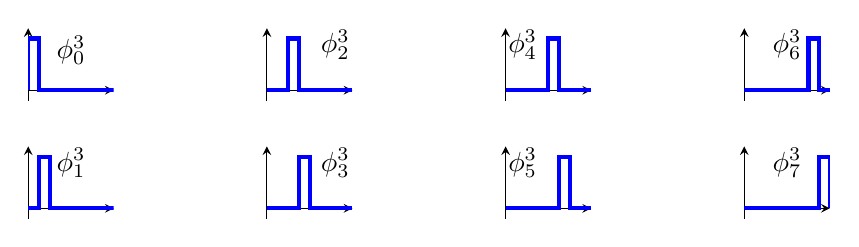
\begin{tikzpicture}
  % Column 1: Scaling functions 1 and 2
  % Scaling function 1: [0, 1/8)
  \begin{axis}[
    at={(0,0)},
    width=0.22\textwidth,
    height=2.5cm,
    xmin=0, xmax=1,
    ymin=-0.2, ymax=1.2,
    ytick=\empty,
    xtick=\empty,
    axis x line=middle,
    axis y line=center,
  ]
    \addplot[const plot, line width=1.5pt, color=blue] coordinates {
      (0,0) (0,1) (0.125,1) (0.125,0) (1,0)
    };
    \node[above] at (0.5, 0.3) {$\phi_0^3$};
  \end{axis}
  % Scaling function 2: [1/8, 1/4)
  \begin{axis}[
    at={(0,-1.5cm)},
    width=0.22\textwidth,
    height=2.5cm,
    xmin=0, xmax=1,
    ymin=-0.2, ymax=1.2,
    ytick=\empty,
    xtick=\empty,
    axis x line=middle,
    axis y line=center,
  ]
    \addplot[const plot, line width=1.5pt, color=blue] coordinates {
      (0,0) (0.125,0) (0.125,1) (0.25,1) (0.25,0) (1,0)
    };
    \node[above] at (0.5, 0.4) {$\phi_1^3$};
  \end{axis}
  
  % Column 2: Scaling functions 3 and 4
  % Scaling function 3: [1/4, 3/8)
  \begin{axis}[
    at={(0.25\textwidth,0)},
    width=0.22\textwidth,
    height=2.5cm,
    xmin=0, xmax=1,
    ymin=-0.2, ymax=1.2,
    ytick=\empty,
    xtick=\empty,
    axis x line=middle,
    axis y line=center,
  ]
    \addplot[const plot, line width=1.5pt, color=blue] coordinates {
      (0,0) (0.25,0) (0.25,1) (0.375,1) (0.375,0) (1,0)
    };
    \node[above] at (0.8, 0.4) {$\phi_2^3$};
  \end{axis}
  % Scaling function 4: [3/8, 1/2)
  \begin{axis}[
    at={(0.25\textwidth,-1.5cm)},
    width=0.22\textwidth,
    height=2.5cm,
    xmin=0, xmax=1,
    ymin=-0.2, ymax=1.2,
    ytick=\empty,
    xtick=\empty,
    axis x line=middle,
    axis y line=center,
  ]
    \addplot[const plot, line width=1.5pt, color=blue] coordinates {
      (0,0) (0.375,0) (0.375,1) (0.5,1) (0.5,0) (1,0)
    };
    \node[above] at (0.8, 0.4) {$\phi_3^3$};
  \end{axis}
  
  % Column 3: Scaling functions 5 and 6
  % Scaling function 5: [1/2, 5/8)
  \begin{axis}[
    at={(0.5\textwidth,0)},
    width=0.22\textwidth,
    height=2.5cm,
    xmin=0, xmax=1,
    ymin=-0.2, ymax=1.2,
    ytick=\empty,
    xtick=\empty,
    axis x line=middle,
    axis y line=center,
  ]
    \addplot[const plot, line width=1.5pt, color=blue] coordinates {
      (0,0) (0.5,0) (0.5,1) (0.625,1) (0.625,0) (1,0)
    };
    \node[above] at (0.2, 0.4) {$\phi_4^3$};
  \end{axis}
  % Scaling function 6: [5/8, 3/4)
  \begin{axis}[
    at={(0.5\textwidth,-1.5cm)},
    width=0.22\textwidth,
    height=2.5cm,
    xmin=0, xmax=1,
    ymin=-0.2, ymax=1.2,
    ytick=\empty,
    xtick=\empty,
    axis x line=middle,
    axis y line=center,
  ]
    \addplot[const plot, line width=1.5pt, color=blue] coordinates {
      (0,0) (0.625,0) (0.625,1) (0.75,1) (0.75,0) (1,0)
    };
    \node[above] at (0.2, 0.4) {$\phi_5^3$};
  \end{axis}
  
  % Column 4: Scaling functions 7 and 8
  % Scaling function 7: [3/4, 7/8)
  \begin{axis}[
    at={(0.75\textwidth,0)},
    width=0.22\textwidth,
    height=2.5cm,
    xmin=0, xmax=1,
    ymin=-0.2, ymax=1.2,
    ytick=\empty,
    xtick=\empty,
    axis x line=middle,
    axis y line=center,
  ]
    \addplot[const plot, line width=1.5pt, color=blue] coordinates {
      (0,0) (0.75,0) (0.75,1) (0.875,1) (0.875,0) (1,0)
    };
    \node[above] at (0.5, 0.4) {$\phi_6^3$};
  \end{axis}
  % Scaling function 8: [7/8, 1)
  \begin{axis}[
    at={(0.75\textwidth,-1.5cm)},
    width=0.22\textwidth,
    height=2.5cm,
    xmin=0, xmax=1,
    ymin=-0.2, ymax=1.2,
    ytick=\empty,
    xtick=\empty,
    axis x line=middle,
    axis y line=center,
  ]
    \addplot[const plot, line width=1.5pt, color=blue] coordinates {
      (0,0) (0.875,0) (0.875,1) (1,1) (1,0)
    };
    \node[above] at (0.5, 0.4) {$\phi_7^3$};
  \end{axis}
\end{tikzpicture}


    \subcaption{Scaling functions (basis) for $V^3$: eight piecewise constant functions.}
    \label{fig:scaling_functions}
  \end{minipage}
  \vspace{0.5cm}
  \begin{minipage}{\textwidth}
    \centering
    % Basis for V_2 (blue) and Haar wavelets basis for W_2 (red)
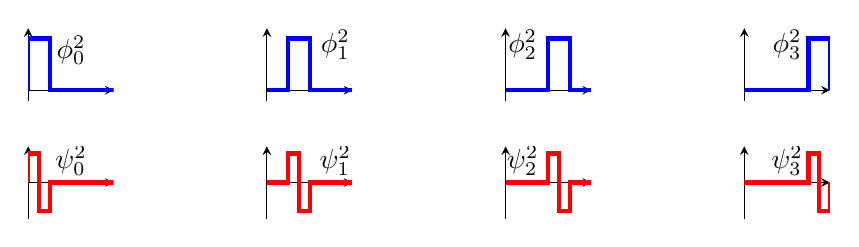
\begin{tikzpicture}
  % V_2 Scaling functions (row above)
  % Scaling function 1: [0, 1/4)
  \begin{axis}[
    at={(0,1.5cm)},
    width=0.22\textwidth,
    height=2.5cm,
    xmin=0, xmax=1,
    ymin=-0.2, ymax=1.2,
    ytick=\empty,
    xtick=\empty,
    axis x line=middle,
    axis y line=center,
  ]
    \addplot[const plot, line width=1.5pt, color=blue] coordinates {
      (0,0) (0,1) (0.25,1) (0.25,0) (1,0)
    };
    \node[above] at (0.5, 0.3) {$\phi_0^2$};
  \end{axis}
  % Scaling function 2: [1/4, 1/2)
  \begin{axis}[
    at={(0.25\textwidth,1.5cm)},
    width=0.22\textwidth,
    height=2.5cm,
    xmin=0, xmax=1,
    ymin=-0.2, ymax=1.2,
    ytick=\empty,
    xtick=\empty,
    axis x line=middle,
    axis y line=center,
  ]
    \addplot[const plot, line width=1.5pt, color=blue] coordinates {
      (0,0) (0.25,0) (0.25,1) (0.5,1) (0.5,0) (1,0)
    };
    \node[above] at (0.8, 0.4) {$\phi_1^2$};
  \end{axis}
  % Scaling function 3: [1/2, 3/4)
  \begin{axis}[
    at={(0.5\textwidth,1.5cm)},
    width=0.22\textwidth,
    height=2.5cm,
    xmin=0, xmax=1,
    ymin=-0.2, ymax=1.2,
    ytick=\empty,
    xtick=\empty,
    axis x line=middle,
    axis y line=center,
  ]
    \addplot[const plot, line width=1.5pt, color=blue] coordinates {
      (0,0) (0.5,0) (0.5,1) (0.75,1) (0.75,0) (1,0)
    };
    \node[above] at (0.2, 0.4) {$\phi_2^2$};
  \end{axis}
  % Scaling function 4: [3/4, 1)
  \begin{axis}[
    at={(0.75\textwidth,1.5cm)},
    width=0.22\textwidth,
    height=2.5cm,
    xmin=0, xmax=1,
    ymin=-0.2, ymax=1.2,
    ytick=\empty,
    xtick=\empty,
    axis x line=middle,
    axis y line=center,
  ]
    \addplot[const plot, line width=1.5pt, color=blue] coordinates {
      (0,0) (0.75,0) (0.75,1) (1,1) (1,0)
    };
    \node[above] at (0.5, 0.4) {$\phi_3^2$};
  \end{axis}
  
  % Wavelet level 2, first: [0, 1/8) vs [1/8, 1/4)
  \begin{axis}[
    at={(0,0)},
    width=0.22\textwidth,
    height=2.5cm,
    xmin=0, xmax=1,
    ymin=-2.5, ymax=2.5,
    ytick=\empty,
    xtick=\empty,
    axis x line=middle,
    axis y line=center,
  ]
    \addplot[const plot, line width=1.5pt, color=red] coordinates {
      (0,0) (0,2) (0.125,2) (0.125,-2) (0.25,-2) (0.25,0) (1,0)
    };
    \node[above] at (0.5, -0.2) {$\psi_0^2$};
  \end{axis}
  % Wavelet level 2, second: [1/4, 3/8) vs [3/8, 1/2)
  \begin{axis}[
    at={(0.25\textwidth,0)},
    width=0.22\textwidth,
    height=2.5cm,
    xmin=0, xmax=1,
    ymin=-2.5, ymax=2.5,
    ytick=\empty,
    xtick=\empty,
    axis x line=middle,
    axis y line=center,
  ]
    \addplot[const plot, line width=1.5pt, color=red] coordinates {
      (0,0) (0.25,0) (0.25,2) (0.375,2) (0.375,-2) (0.5,-2) (0.5,0) (1,0)
    };
    \node[above] at (0.8, -0.2) {$\psi_1^2$};
  \end{axis}
  % Wavelet level 2, third: [1/2, 5/8) vs [5/8, 3/4)
  \begin{axis}[
    at={(0.5\textwidth,0)},
    width=0.22\textwidth,
    height=2.5cm,
    xmin=0, xmax=1,
    ymin=-2.5, ymax=2.5,
    ytick=\empty,
    xtick=\empty,
    axis x line=middle,
    axis y line=center,
  ]
    \addplot[const plot, line width=1.5pt, color=red] coordinates {
      (0,0) (0.5,0) (0.5,2) (0.625,2) (0.625,-2) (0.75,-2) (0.75,0) (1,0)
    };
    \node[above] at (0.2, -0.2) {$\psi_2^2$};
  \end{axis}
  % Wavelet level 2, fourth: [3/4, 7/8) vs [7/8, 1)
  \begin{axis}[
    at={(0.75\textwidth,0)},
    width=0.22\textwidth,
    height=2.5cm,
    xmin=0, xmax=1,
    ymin=-2.5, ymax=2.5,
    ytick=\empty,
    xtick=\empty,
    axis x line=middle,
    axis y line=center,
  ]
    \addplot[const plot, line width=1.5pt, color=red] coordinates {
      (0,0) (0.75,0) (0.75,2) (0.875,2) (0.875,-2) (1,-2) (1,0)
    };
    \node[above] at (0.5, -0.2) {$\psi_3^2$};
  \end{axis}
\end{tikzpicture}


    \subcaption{Basis for $V^2$ (blue) and Haar wavelets basis for $W^2$ (red).}
    \label{fig:wavelet_basis}
  \end{minipage}
  \caption{Haar basis: scaling functions for $V^3$ and scaling functions and wavelets for $V^2$ and $W^2$.}
  \label{fig:basis_functions}
\end{figure*}

A detailed mathematical exposition of the vector space structure, scaling functions, inner products, orthogonality, and the Haar wavelet basis functions is provided in Appendix \ref{apx:haartheory}.




\subsubsection{Two-Dimensional Haar Wavelet Transform}

The 2D Haar wavelet transform generalizes the 1D "averaging and differencing" filter bank to 2D by alternating between operations on rows and columns at each level of the hierarchy.

\paragraph{The Decomposition Algorithm}

The algorithm proceeds recursively as follows:

\begin{enumerate}
\item \textbf{Row Step:} First, perform one step of horizontal pairwise averaging and differencing on the pixel values in each row of the image. This splits the image horizontally into averages (left) and details (right).

\item \textbf{Column Step:} Next, apply vertical pairwise averaging and differencing to each column of the result from the Row Step.
\begin{itemize}
\item This creates four distinct quadrants of coefficients:
\begin{itemize}
\item \textbf{Top-Left:} Averages of averages (coarse approximation).
\item \textbf{Top-Right:} Averages of horizontal details.
\item \textbf{Bottom-Left:} Vertical details of horizontal averages.
\item \textbf{Bottom-Right:} Vertical details of horizontal details (diagonal details).
\end{itemize}
\end{itemize}

\item \textbf{Recursion:} To complete the transformation, repeat this process recursively \textit{only} on the quadrant containing the averages in both directions (the top-left quadrant).
\end{enumerate}

Figure~\ref{fig:encoded_visualization} visualizes this 2D Haar transform decomposition process, showing how an image is decomposed into four quadrants at each level.

\begin{figure}[ht]
  \centering
  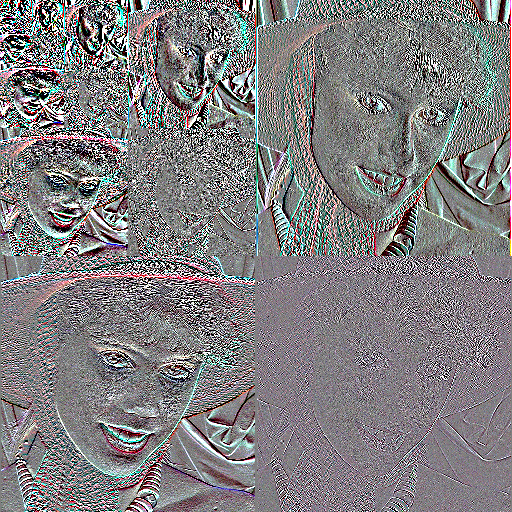
\includegraphics[width=0.3\textwidth]{methods/DWTdiagrams/encodedVisualization.png}
  \caption{Visualization of a 2D Haar transform showing the decomposition of an image}
  \label{fig:encoded_visualization}
\end{figure}




\subsubsection{Compression Properties}

The Haar wavelet transform is particularly effective for image compression because it naturally concentrates energy in the low-resolution approximation coefficients. The detail coefficients (wavelets) typically have smaller magnitudes and can be more aggressively quantized or discarded in lossy compression scenarios. This energy compaction property, combined with the transform's computational efficiency makes the Haar wavelet an attractive choice for practical image compression systems.

